\section{コレクションを更新する}

私たちのアプリケーションは、新しい情報を受け取り、既存の情報を更新し、不要になった情報を削除するなど、常に外部と通信しています。しかし、これはClojureのイミュータブルなコア・コレクションと相反するように思えます。

Clojureでは、変化は常に純粋な関数をイミュータブルな値に適用し、その結果新しいイミュータブルな値が得られるというモデルになっています。言語学的なごまかしを避けるため、この変更手段を説明するために、単純な更新という言葉を使うことにします。

コレクションをイミュータブルに定義することには、多くの利点がある。まず、同時実行スレッドでは、値への参照ではなく、値の受け渡しが可能になる。これにより、他のスレッドによってデータが予測不可能に変更されることがない。第二に、ドメインロジックを状態管理機能から分離し、並行処理に関する問題をドメインデータや関数からきれいに分離します。

シーケンシャルなデータで発生する特殊なケースとして、キューのようにデータを更新する必要があります(先入れ先出し処理とも呼ばれる)。

\subsection{先入先出の処理}

ランチカウンターで、店員から注文が来ることを想像してください。公平性を保つために、注文は受け取った順に処理されることが期待されている - 先入れ先出し (FIFO) 処理。

Clojureでランチ・カウンターをモデル化するには、保留中のランチ・オーダーを保持するためのコレクションが必要です。ランチ・オーダーは時間的に自然な順序を持つので、リストやベクターのような連続したコレクションが必要なことが分かっています。ベクターを試してみましょう。

\begin{lstlisting}[numbers=none]
(defn new-orders [] [])

(defn add-order [orders order]
  (conj orders order))

(defn cook-order [orders]
  (cook (first orders)) (rest orders))
\end{lstlisting}

\texttt{add-order}関数は、\texttt{orders}の末尾に新しい\texttt{order}を追加しているので、vectorとしては効率的です。しかし、\texttt{orders}ベクターに対して\texttt{rest}を呼び出すのは非効率的です。これは、最初の要素以外のすべてを含むシーケンス(ベクターではない)を作成し、それを返します。もしベクターコレクション型を維持したければ、新しいベクターを構築し、そこにシーケンス要素を追加し直す必要があります;このすべてが高価です。

また、\texttt{orders}をリストで実装することもできる。\texttt{cook-order} のコードはそのままです。しかし、リンクされたリスト上で \texttt{rest} を呼び出すと効率的なので、ベクターで起こったパフォーマンスの問題に対処しています。しかし、\texttt{add-order}では新たな問題が発生しました。

\begin{lstlisting}[numbers=none]
(defn new-orders [] '())

(defn add-order [orders order]
  (concat orders (list order)))
\end{lstlisting}

リストの末尾にオブジェクトを追加する場合、リスト全体を走査して最後の要素を見つけ、新しいポインタを追加する必要があります。リストは先頭でのみ、ベクターは末尾でのみ効率的に追加と削除を行います。しかし、最後に追加し、最初に削除するコレクションが必要である。このニーズに応えるのが、次の図に示すようなキュー(待ち行列)です。

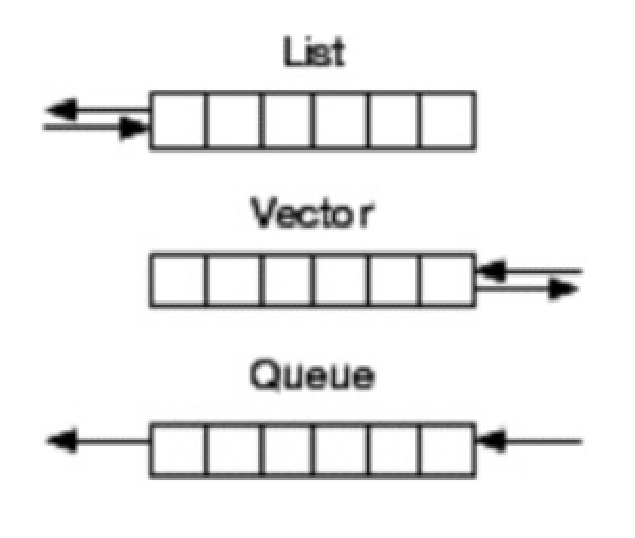
\includegraphics[width=5cm]{fig_02_001.eps}


他のすべてのコアコレクションと同様に、キューは不変の永続的なコレクションであり、リストやベクトルを扱うのと同じ関数をすべてサポートしています。以下は、ランチカウンターをキューで実装する方法です。

\begin{lstlisting}[numbers=none]
(def new-orders clojure.lang.PersistentQueue/EMPTY)

(defn add-order [orders order]
  (conj orders order))

(defn cook-order [orders]
  (cook (peek orders))
  (pop orders))
\end{lstlisting}

Clojureはリテラルなキューの構文やコンストラクタを提供しません。新しいキューを作成するには、静的な空のインスタンス \texttt{clojure.lang.PersistentQueue/EMPTY} で開始します。\texttt{add-order}では、vectorのように最後に新しい要素を追加するために\texttt{conj}を使用するだけです。\texttt{cook-order}では、最初の順序を見るために\texttt{peek}を使い、最初の順序以外を返すために\texttt{pop}を使います。

待ち行列の実装は、順序の追加と、待ち行列に入れられた順序での順序の削除の両方において効率的です。これは、この仕事に適したツールです。

次に、コレクションにデータを追加する処理を最適化する方法を考えてみましょう。


\subsection{一括インポート}

Clojureの永続的なコレクションは、イミュータブルです。効率化のために、\texttt{conj}や\texttt{assoc}のような関数で要素を追加すると、新しい不変の構造が作成されますが、その前と後のバージョンは通常そのデータの多くを共有します。コレクションは不変なので、これは安全に実行でき、データをコピーするよりもはるかに高速です。しかし、Clojureは制御されたコンテキストでミュータビリティを活用することで、より効率的にコレクションを埋める方法があります。

典型的なケースは、カタログアイテムのインポートです。アプリケーションが記録システムに直接アクセスできない場合、そのシステムからのエクスポートは、開始時にアプリケーションにインポートすることができます。カタログが変更されると、定期的な更新が必要になることは容易に想像できる。大規模なカタログの場合、その処理には時間がかかることがあります。

アプリケーションの起動時に呼び出される典型的なインポートを考えてみましょう。


\begin{lstlisting}[numbers=none]

\end{lstlisting}








\begin{lstlisting}[numbers=none]

\end{lstlisting}





